% \chapter{Линейная регрессия. Продолжение.}\label{cha:linreg2}

\newpage
\begin{problem}
	В файле $ "House\_prices.csv"  $ представлены характеристики различных домов (стоимость, площадь, количество комнат, год постройки и тп, описание признаков можно найти по ссылке Ames Housing dataset).

	Изучить линейную зависимость стоимости домов (SalePrice) от всех остальных показателей.
\end{problem}
\begin{lstlisting}[language=Python][frame=single]
	import numpy as np
	import scipy as sp
	import pandas as pd
	import matplotlib.pyplot as plt
	import scipy.stats as st
	import seaborn as sns
	sns.set()
	from statsmodels.regression.linear_model import OLS
	from statsmodels.tools.tools import add_constant
	from scipy.stats import probplot
	from scipy.stats import jarque_bera
	from sklearn.metrics import mean_squared_error, r2_score
	from sklearn.linear_model import LinearRegression
	from sklearn.model_selection import train_test_split
	from sklearn.model_selection import cross_val_score
	from sklearn.metrics import make_scorer
	
	data = pd.read_csv('House_prices.csv')
\end{lstlisting}

\section{Пропуски в данных}\label{cha:linreg2/sec:propuski}

% \subsection{Пропуски в данных.}\label{cha:linreg2}
	Часто в реальных данных не для всех объектов известно значение того или иного признака. Такие объекты нужно обрабатывать прежде, чем приступать к построению линейной регрессии. Для каждого признака посмотрим, в какой доле объектов отсутствует значение. Пропуски заполним медианным значением
	
\begin{lstlisting}[language=Python][frame=single]
	fill = data.median(axis=0) #axis=0: по столбцам
	data = data.fillna(value=fill)
\end{lstlisting}

\section{Проверка на мультиколлинеарность}\label{cha:linreg2/sec:multi}

% \subsection{Проверка на мультиколлинеарность.}\label{cha:linreg2}
	Посмотрим на матрицу корреляций признаков и целевой переменной SalePrice
	
\begin{lstlisting}[language=Python][frame=single]
	corr = data.corr()
	plt.figure(figsize=(15, 11))
	sns.heatmap(corr, vmax=.8, square=True, cmap='magma');
\end{lstlisting}
\begin{center}
	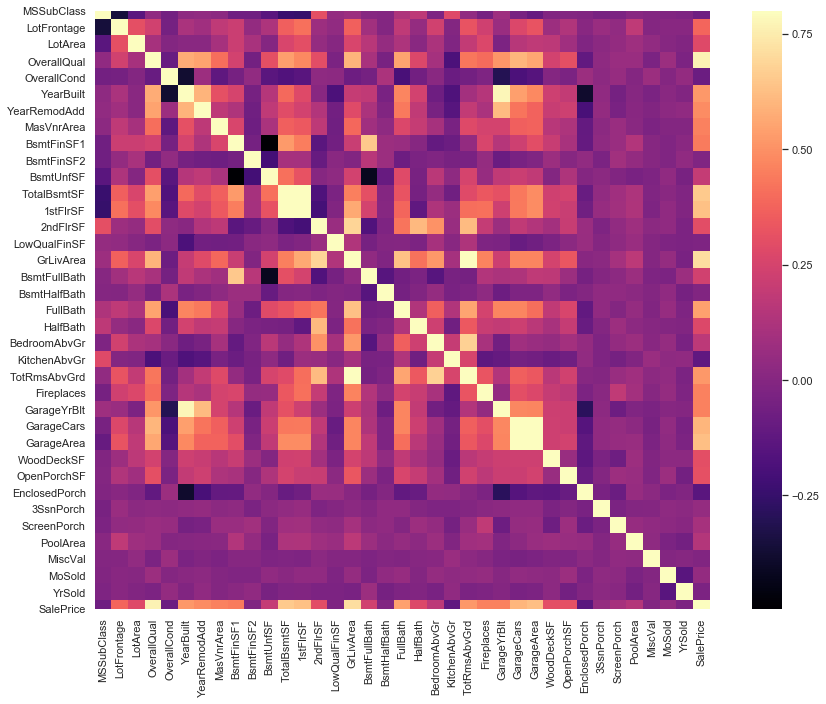
\includegraphics[scale=0.6]{multicoll} 
\end{center}

	Чем светлее ячейка, соответствующая паре признаков $ (feature_i, feature_j) $, тем больше корелляция между ними.
	
	Посмотим значения корелляций в численном виде.
	
\begin{lstlisting}[language=Python][frame=single]
	corr_df = corr.unstack().to_frame().reset_index() 
	#corr.unstack(): сделали двухуровневый индекс, получили series (1 столбец со сложным индексом)
	#reset_index(): превратили индекс в значения ячеек
	new_coor_table = corr_df[corr_df.level_0!=corr_df.level_1].sort_values(0, ascending=False)
	#corr_df.level_0!=corr_df.level_1 : убираем пары с одинаковыми признаками
\end{lstlisting}

	Если есть сильно скоррелированны, то выбросим из каждой пары по одному признаку. Например, хотим выбросить признаки 'TotalBsmtSF', 'GarageYrBlt', 'GarageCars', 'TotRmsAbvGrd', тогда:

\begin{lstlisting}[language=Python][frame=single]
	data.drop(['TotalBsmtSF', 'GarageYrBlt', 'GarageCars', 'TotRmsAbvGrd'], 1, inplace=True)
\end{lstlisting}

	Строим регрессию.
	
\begin{lstlisting}[language=Python][frame=single]
	x = add_constant(data.drop(['SalePrice'], 1))
	y = data['SalePrice']
	ols = OLS(y, x)
	results = ols.fit()
	RSS = results.ssr
	n, k = x.shape[0], x.shape[1]
	sigma2_hat = RSS/(n-k)
\end{lstlisting}

	Проверим остатки на нормальность:
	
\begin{lstlisting}[language=Python][frame=single]
	probplot(stand_residuals, plot=plt);
	sns.boxplot(data=stand_residuals, orient="h");
\end{lstlisting}

\begin{figure}[h]
  \caption{probplot}
  \centering
    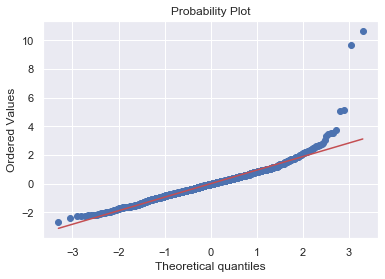
\includegraphics[scale=0.6]{qqplot}
\end{figure}
\begin{figure}[h]
  \caption{boxplot}
  \centering
    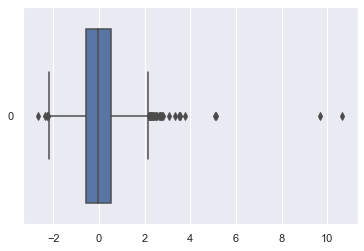
\includegraphics[scale=0.6]{boxplot}
\end{figure}

	Видим, что не очень хорошо все ложится на прямую в случае qqplot, для boxplot есть выбросы $ \Longrightarrow $ есть подозрения на невыаолнение условия нормальности остатков. Разочаруемся в предположении о нормальности до конца:

\begin{lstlisting}[language=Python][frame=single]
	jarque_bera(stand_residuals)
\end{lstlisting}

	Результат : $ Jarque\_beraResult(statistic=16543.863883530954, pvalue=0.0) $, то есть остатки не есть нормальные. Если не хотим применять результаты нормальное регрессии, то это не проблема. Что делать в ином случае? Преобразуем данные: пытаемся брать логорифмы, експоненту и т.д. в надежде на то, что новая реграссия будет удовлетворять условиям нормальности. Можно применить преобразование Бокса - Кокса. Чаще всего используют логарифм.

\begin{lstlisting}[language=Python][frame=single]
	ln_y = np.log(y)
	ln_ols = OLS(ln_y, x)
	ln_results = ln_ols.fit()
	ln_RSS = ln_results.ssr
	n, k = x.shape[0], x.shape[1]
	ln_sigma2_hat = ln_RSS/(n-k)
	ln_influence = ln_results.get_influence()
	ln_residuals = ln_influence.resid
	ln_stand_residuals = ln_residuals/np.sqrt(ln_sigma2_hat)
	probplot(ln_stand_residuals, plot=plt);
	sns.boxplot(data=ln_stand_residuals, orient="h");
	jarque_bera(ln_stand_residuals)
\end{lstlisting}

\begin{figure}[h]
  \caption{probplot}
  \centering
    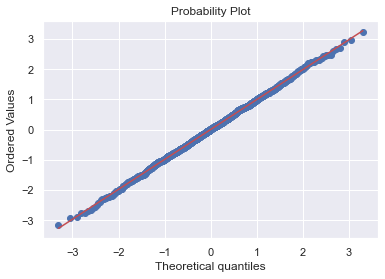
\includegraphics[scale=0.6]{qqplot_ln}
\end{figure}
\begin{figure}[h]
  \caption{boxplot}
  \centering
    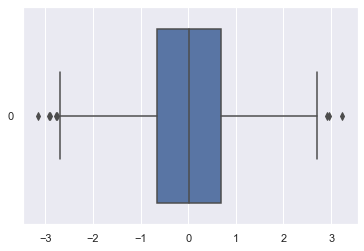
\includegraphics[scale=0.6]{boxplot_ln}
\end{figure}

	Результат теста Харке - Бера: $ Jarque\_beraResult(statistic=0.06510310527385516, pvalue=0.9679725470077343) $, то есть теперь имеем нормальную регрессию.

\begin{remark}
	Помним о том, что мы работаем с логарифмом регрессии, поэтому, когда хотим проводить какие-либо сравнения с исходными данными, необходимо произвести обратное преобразование.
\end{remark}

\section{Отбор признаков. Информационные критерии AIC и BIC}\label{cha:linreg2/sec:otbor+aic+bic}

% \subsection{Отбор признаков.Информационные критерии AIC и BIC.}\label{cha:linreg2}
 
 	Хотим отобрать признаки, для этого нам необходимо сравнивать модели, построенные на разных наборах признаков $ \lbrace x_{i_k} \rbrace_k $ и $ \lbrace x_{i_s} \rbrace_s $. Для этого используются информационные критерии AIC (информационный критерий Акаике) и BIC (Байесовский информационный критерий):
$$\begin{gathered}
  AIC = 2k + n\log(RSS) ,\\
  BIC = \log(n)k + n\log(RSS),
\end{gathered}$$
	где $ RSS = \sum\limits_{i = 1}^n (x_i - \hat{x}_i)^2, \;  \hat{x}_i = z_i\hat{\theta}, \; \hat{\theta} = (Z^TZ)^{-1}Z^TX, \; X = (x_1, \ldots, x_n)$  -- вектор наблюдений, $ Z = (z_{ik}) $ -- матрица факторов (факторов k штук, имеем n наблюдений). Модель с меньшим AIC/BIC - лучшая.
	
\begin{remark}
	Из формулы для подсчета AIC и BIC видно, что BIC штрафует за добавление новых признаков сильнее, чем AIC, поэтому подбор признаков, основанный на BIC, как правило, всегда исключает больше признаков, чем при подборе признаков, основанном на AIC.
\end{remark}

\begin{remark}
	Данные формулы лучше использовать для нормальной регрессии.
\end{remark}
	
\begin{lstlisting}[language=Python][frame=single]
	def select_best_combination(y, x, metric): #metric: 'aic' или 'bic'
    current_factors = x.columns.to_list() #сначала создаем список всех наименований столбцов
    ols = OLS(y, x[current_factors]) 
    results = ols.fit()
    metric_base = getattr(results, metric) 

    while 1 == 1:
        res = pd.Series(index=current_factors) #создаем Series c индексом current_factors и значениями = Nan
        for factor in current_factors:
            ols = OLS(y, x[list(set(current_factors)-{factor})]) #выкидываем по очереди один столбец
            results = ols.fit()
            res.loc[factor] = getattr(results, metric) #вместо Nan в res записываем метрику, соответствующую модели без данного столбца
        res = res.sort_values(ascending=True) #сортируем res по возрастанию 
        if res.iloc[0] < metric_base:
            current_factors.remove(res.index.values[0])
            metric_base = res.iloc[0]
        else:
            break
            
    ols = OLS(y, x[current_factors])
    results = ols.fit()
    
    return current_factors, results
    
    current_factors, results = select_best_combination(ln_y, x, 'bic')
    set(x.columns.to_list()) - set(current_factors) #вывод факторов, основываясь на BIC
    current_factors, results = select_best_combination(ln_y, x, 'aic')
    set(x.columns.to_list()) - set(current_factors) #вывод факторов, основываясь на AIC
\end{lstlisting}

\section{Деление выборки на обучающую и тестовую}\label{cha:linreg2/sec:train+test}

% \subsection{Деление выборки на обучающую и тестовую.}\label{cha:linreg2}

	Разделим выборку на обучающую и тестовую. Разделим случайным образом 75$ \% $ на 25$ \% $:

\begin{lstlisting}[language=Python][frame=single]
	x_train, x_test, y_train, y_test = train_test_split(x, y, test_size=0.25, random_state=10)
\end{lstlisting}

	У моделей из sklearn есть методы fit и predict. fit принимает на вход обучающую выборку и вектор целевых переменных и обучает модель, predict, будучи вызванным после обучения модели, возвращает предсказание на выборке.

\begin{lstlisting}[language=Python][frame=single]
	lr = LinearRegression() #по умолчанию в модели регрессии есть константа
	lr.fit(x_train, y_train)

	y_hat_test = lr.predict(x_test)
	print('Using Y:')
	print('Test MSE %.3f' % mean_squared_error(y_test, y_hat_test))
	print('Test R2 %.3f' % r2_score(y_test, y_hat_test))
	
	y_hat_train = lr.predict(x_train)
	print("Train MSE = %.3f" % mean_squared_error(y_train, y_hat_train))
	print("Train R2 = %.3f" % r2_score(y_train, y_hat_train)) 
\end{lstlisting}

	Вывод:  
	
	Using Y:
	
	Test MSE 1304270005.734
	
	Test R2 0.771
	
	Train MSE = 1342194893.254
	
	Train R2 = 0.813
	
	Если будем использовать логарифмирование данных, получим

\begin{lstlisting}[language=Python][frame=single]
	lr.fit(x_train, np.log(y_train))
	y_hat_test = np.exp(lr.predict(x_test))
	print('Using logY:')
	print('Test MSE %.3f' % mean_squared_error(y_test, y_hat_test))
	print('Test R2 %.3f' % r2_score(y_test, y_hat_test))
\end{lstlisting}

	Вывод:
	
	Using logY:
	
	Test MSE 866920715.293
	
	Test R2 0.848

	Итак, мы обучили модель и посчитали ее качество на тестовой выборке. 

\section{Кросс-валидация}\label{cha:linreg2/sec:crossvalid}

% \subsection{Кросс-валидация.}\label{cha:linreg2}

	Принцип кросс-валидации изображен на рисунке. Берем данные, делим на k групп равного объема (k -- количество фолдов). Делаем все то же самое, что ранее для train и test k раз: для i-го фолда $ i = 1,\ldots,k $ считаем метрику $ metric_i  $ на $ test_i $. Итоговое значение качества модели по кросс - валидации есть значение.
	
$$\begin{gathered} 
\dfrac{\sum\limits_{i =1}^kmetric_i}{k}.
\end{gathered} $$

\begin{figure}[h]
  \caption{5 фолдов}
  \centering
    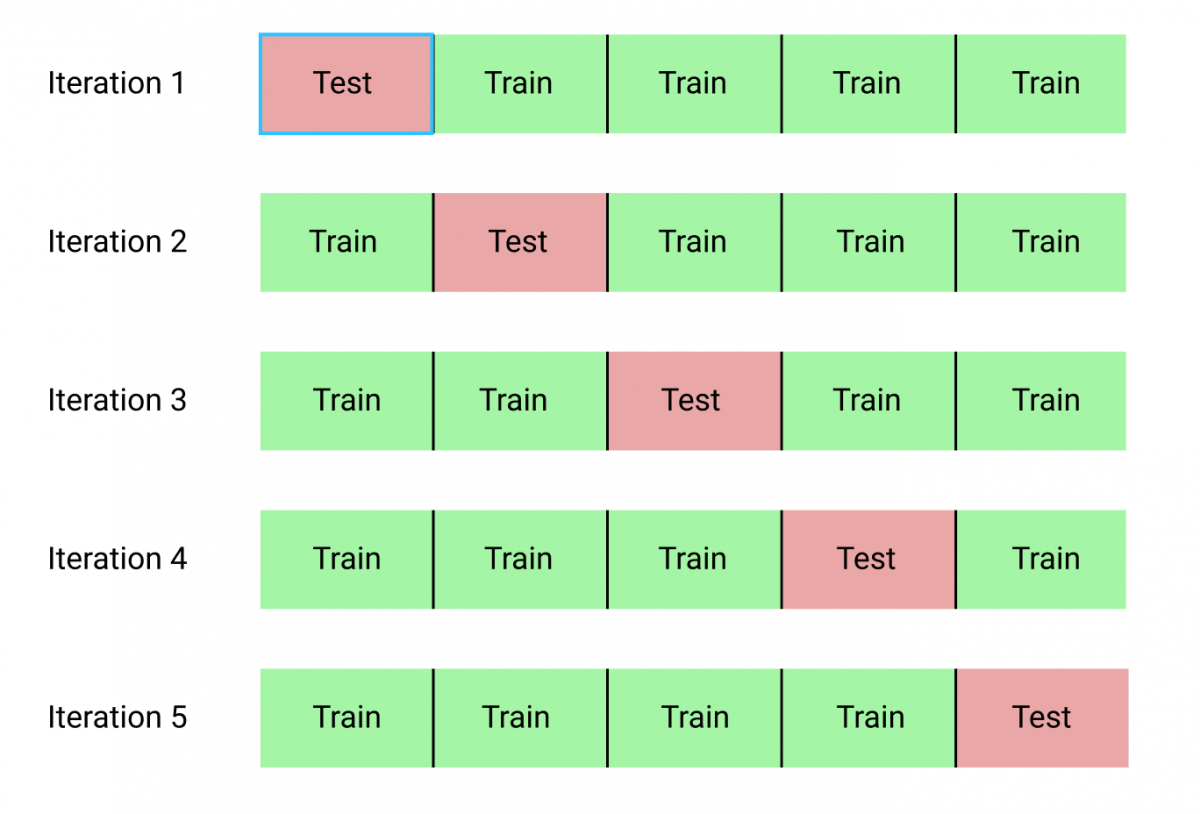
\includegraphics[scale=0.4]{cross_val}
\end{figure}

\begin{lstlisting}[language=Python][frame=single]
	cv_scores = cross_val_score(lr, x, y, cv=10, scoring="neg_mean_squared_error")
\end{lstlisting}

	Если мы выведем $ cv\_scores  $, то результаты получились отрицательными. Это соглашение в sklearn (скоринговую функцию нужно максимизировать). Поэтому все стандартные скореры называются $ neg\_* $, например, $ neg\_mean\_squared\_error  $.
	
\begin{lstlisting}[language=Python][frame=single]
	print("Mean CV MSE = %.4f" % np.mean(-cv_scores)) #итоговое значение качества модели по кросс - валидации
\end{lstlisting}

	В нашем примере она равна Mean CV MSE = 1494450970.6308. Мы всегда можем определить свою метрику и использовать ее, например, в $ cross\_val\_score $. Для этого нужно воспользоваться $ sklearn.metrics.make\_scorer $. Ниже показано, как можно задать свою метрику на примере метрики $ R^2 $ (на самом деле, она прописана в sklearn: $ \# $scoring="r2" в функции $ cross\_val\_score $)
	
\begin{lstlisting}[language=Python][frame=single]
	def r2_squared(y_true, y_pred):
    r2_coef = r2_score(y_true, y_pred)
    return r2_coef

	r2_scorer = make_scorer(r2_squared, greater_is_better=True) #greater_is_better влияет на знаки метрик в cv_scores
	cv_scores = cross_val_score(lr, x, y, cv=10, scoring=r2_scorer) 
	print("Mean CV R2 = %.4f" % np.mean(cv_scores))
	
	cv_scores = cross_val_score(lr, x, ln_y, cv=10, scoring=r2_scorer) 
	print("Mean CV R2 = %.4f" % np.mean(cv_scores))
\end{lstlisting}

	Вывод для не логарифма: Mean CV R2 = 0.7825. Для $ \log y:$  Mean CV R2 = 0.8504.

\subsection{Отбор признаков с помощью кросс-валидации (greedy algorithm)}\label{cha:linreg2/subsec:greedy}

% \subsection{Отбор признаков с помощью кросс-валидации (greedy algorithm).}\label{cha:linreg2}

	Вместо критериев AIC и BIC возьмем итоговое значение качества модели по кросс - валидации:

\begin{lstlisting}[language=Python][frame=single]
def calc_kfold_validation(x, y):
    lr = LinearRegression()
    cv_scores = cross_val_score(lr, x, y, cv=5, scoring="neg_mean_squared_error")
    return np.mean(-cv_scores)
    
def select_best_combination(x, y):
    current_factors = x.columns.to_list() #сначала создаем список всех наименований столбцов
    metric_base = calc_kfold_validation(x[current_factors], y)

    while 1 == 1:
        res = pd.Series(index=current_factors) #создаем Series c индексом current_factors и значениями = Nan
        for factor in current_factors:
            res.loc[factor] = calc_kfold_validation(x[list(set(current_factors)-{factor})], y)
                #вместо Nan в res записываем метрику, соответствующую модели без данного столбца
        res = res.sort_values(ascending=True) #сортируем res по возрастанию 
        if res.iloc[0] < metric_base:
            current_factors.remove(res.index.values[0])
            metric_base = res.iloc[0]
        else:
            break
            
    return current_factors, calc_kfold_validation(x[current_factors], y)
    
 ln_y_train, ln_y_test = np.log(y_train), np.log(y_test)
 current_factors, _ = select_best_combination(x_train, ln_y_train) #делаем отбор признаков на train (по ln_y_train)
 set(x.columns.to_list()) - set(current_factors)
\end{lstlisting}

\subsection*{Сравним модель до и после отбора признаков.}\label{cha:linreg2}

\begin{lstlisting}[language=Python][frame=single]
	k = x_train.shape[1] + 1 #количество факторов (с учетом const)
	n = x_test.shape[0]
	lr = LinearRegression()
	lr.fit(x_train, ln_y_train)

	ln_y_hat_test = lr.predict(x_test)
	print('Test R2 %.3f' % r2_score(ln_y_test, ln_y_hat_test))
	print('Test AIC %.3f' % (2*k + n * np.log(np.sum((ln_y_test - ln_y_hat_test) ** 2))) )
\end{lstlisting}

	Вывод:
	
	Test R2 0.858
	
	Test AIC 835.847

\begin{lstlisting}[language=Python][frame=single]
	k = x_train[current_factors].shape[1] + 1 #количество факторов (с учетом const)
	n = x_test.shape[0]
	lr = LinearRegression()
	lr.fit(x_train[current_factors], ln_y_train)

	ln_y_hat_test = lr.predict(x_test[current_factors])
	print('After greedy algorithm')
	print('Test R2 %.3f' % r2_score(ln_y_test, ln_y_hat_test))
	print('Test AIC %.3f' % (2*k + n * np.log(np.sum((ln_y_test - ln_y_hat_test) ** 2))) )
\end{lstlisting}

	Вывод:
	
	After greedy algorithm
	
	Test R2 0.856
	
	Test AIC 821.092

\section{Гребневая регрессия}\label{cha:linreg2/sec:greb}

Было: $\displaystyle X_i = \theta_1 + Z_{i2}\theta_2 + \dots + Z_{ik} \theta_k + \varepsilon_i = <Z_i, \theta> + \varepsilon_i$.

МНК: $\displaystyle S(\theta) = \left( X - Z \theta \right)^T \left( X - Z \theta \right) \to \underset{\theta}{\min}$.

\begin{theorem}[]\label{lec:greb/the:}
	Если $A = Z^T Z$ не вырождена, то $\exists !$ о.н.к. $\hat{\theta} = \left( Z^T Z \right)^{-1} Z^T X$.
\end{theorem}

Если $A$ необратима, то мы получаем проблему мультиколлинераности, то имеются коррелирующие (линейно зависимые) признаки. Т.е. если $A$ не обратима, то задача $S(\theta) \to \min$ имеет бесконечное число решений, то регрессия получается переобученная.\\
Т.к. $\exists$ линейная зависимость признаков, то $\exists$ вектор $\lambda: \; <Z_i, \lambda> = 0 \; \forall i \; \Rightarrow$
$$\begin{gathered}
	X_i = <\theta, Z_i> + \varepsilon_i \\
	<\hat{\theta} + c \lambda, Z_i> = <\hat{\theta}, Z_i> + c \cdot \underbrace{\sqrt{<\lambda, Z_i>}}_{=0} = <\hat{\theta}, Z_i>
\end{gathered}$$

\section{Регуляризация}\label{cha:linreg2/sec:regul}

Вместо задачи минимизации $S(\theta)$ рассматривается минимизация следующего функицонала:
$$\begin{gathered}
	S_{\alpha} = S(\theta) + \alpha \cdot R(\theta) \to \underset{\theta}{\min} \\
	\text{где } \alpha \text{ - параметр, } R(\theta) \text{ - регуляризатор}
\end{gathered}$$
$L_2: \; R(\theta) = \underset{j=2}{\overset{k}{\sum}}\theta_j^2$ - получаем гребневую регрессию. \\
$L_1: \; R(\theta) = \underset{j=2}{\overset{k}{\sum}}|\theta_j|$.\\

В случае $L_2$ регуляризации $\displaystyle \hat{\theta} = \left( Z^T Z + \alpha \cdot \mathbb{I} \right)^{-1} Z^T X$.

В sklearn есть несколько классов, реализующих линейную регрессию:
\begin{enumerate}
	\item LinearRegression — <<классическая>> линейная регрессия с оптимизацией MSE
	\item Ridge — линейная регрессия с оптимизацией MSE и $l_2$-регуляризацией
	\item Lasso — линейная регрессия с оптимизацией MSE и $l_1$-регуляризацией
\end{enumerate}

\begin{lstlisting}[language=Python]
	lr = LinearRegression()
	lr = Ridge() #по умолчанию alpha=1.0, fit_intercept=True
	lr.fit(x_train, y_train)

	y_hat_test = lr.predict(x_test)
	print('Test MSE %.3f' % mean_squared_error(y_test, y_hat_test))
	print('Test R2 %.3f' % r2_score(y_test, y_hat_test))

	#для сравнения
	y_hat_train = lr.predict(x_train)
	print("Train MSE = %.3f" % mean_squared_error(y_train, y_hat_train))
	print("Train R2 = %.3f" % r2_score(y_train, y_hat_train))
\end{lstlisting}

\section{Отбор признаков}\label{cha:linreg2/sec:otborprizn}

Посмотрим на то, какие признаки оказались самыми "сильными". Для этого визуализируем коэффициенты регрессии, соответствующие признакам.

\begin{lstlisting}[language=Python]
	sorted(zip(a, b, c), reverse=True) #сортировка по 1ым элементам по убыванию

	def show_weights(features, weights, scales):
	    fig, axs = plt.subplots(figsize=(14, 10), ncols=2) #ncols=2: два графика (два столбца)
	    sorted_weights = sorted(zip(weights, features, scales), reverse=True) #сортировка по весам по убыванию
	    weights = [x[0] for x in sorted_weights]
	    features = [x[1] for x in sorted_weights]
	    scales = [x[2] for x in sorted_weights]
	    sns.barplot(y=features, x=weights, ax=axs[0])
	    axs[0].set_xlabel("Weight")
	    sns.barplot(y=features, x=scales, ax=axs[1])
	    axs[1].set_xlabel("Scale")
	    plt.tight_layout()

	show_weights(x_train.columns, lr.coef_, x_train.std())
\end{lstlisting}

Будем масштабировать наши признаки. Это сделает нашу регуляризацию более честной: теперь все признаки будут регуляризоваться в равной степени.

Для этого воспользуемся трансформером StandardScaler. Трансформеры в sklearn имеют методы fit и transform (а еще fittransform). Метод fit принимает на вход обучающую выборку и считает по ней необходимые значения (среднее и стандартное отклонение каждого из признаков). transform применяет преобразование к переданной выборке.

\begin{lstlisting}[language=Python]
	scaler = StandardScaler()
	x_train_scaled = scaler.fit_transform(x_train)
	x_test_scaled = scaler.transform(x_test) #на test делаем только transform!

	lr = Ridge()
	lr.fit(x_train_scaled, y_train)

	show_weights(x_train.columns, lr.coef_, x_train_scaled.std(axis=0)) #type(x_train_scaled
\end{lstlisting}

\section{Подбор гиперпараметров}\label{cha:linreg2/sec:hyperpar}

Наряду с параметрами, которые модель оптимизирует на этапе обучения (коэффициенты регрессии), у модели есть и гиперпараметры. У нашей модели это alpha — коэффициент регуляризации.

Будем пользоваться кросс-валидацией для подбора гиперпараметров.

Подберем alpha по логарифмической сетке, чтобы узнать оптимальный порядок величины.

\begin{lstlisting}[language=Python]
	from sklearn.metrics import make_scorer

	def r2_squared(y_true, y_pred):
	    r2_coef = r2_score(y_true, y_pred)
	    return r2_coef

	r2_scorer = make_scorer(r2_squared, greater_is_better=True)

	alphas = np.logspace(-2, 3, 20)
	searcher = GridSearchCV(Ridge(), [{"alpha": alphas}], scoring=r2_scorer, cv=10) #scoring="r2"
	searcher.fit(x_train_scaled, y_train)

	best_alpha = searcher.best_params_["alpha"]
	print("Best alpha = %.4f" % best_alpha)

	plt.plot(alphas, searcher.cv_results_["mean_test_score"])
	plt.xscale("log")
	plt.xlabel("alpha")
	plt.ylabel("CV score")

	lr = Ridge(best_alpha) 
	lr.fit(x_train_scaled, y_train)

	y_hat_test = lr.predict(x_test_scaled)
	print('Test MSE %.3f' % mean_squared_error(y_test, y_hat_test))
	print('Test R2 %.3f' % r2_score(y_test, y_hat_test))

	lr.intercept_

	lr = Ridge() 
	lr.fit(x_train_scaled, y_train)

	y_hat_test = lr.predict(x_test_scaled)
	print('Test MSE %.3f' % mean_squared_error(y_test, y_hat_test))
	print('Test R2 %.3f' % r2_score(y_test, y_hat_test))

	lr.intercept_ #обратим внимание на то, что константа в регрессии не регуляризуется
\end{lstlisting}

\subsection*{Пример}\label{cha:linreg2/subsec:prob}

\begin{problem}
	В файле <<House-prices-corrected.csv>> представлены характеристики различных домов (стоимость, площадь, количество комнат, год постройки и тп, описание признаков можно найти по ссылке Ames Housing dataset).
	
	Изучить линейную зависимость стоимости домов (SalePrice) от всех остальных показателей.
\end{problem}

\begin{lstlisting}[language=Python]
	#from sklearn.linear_model import LinearRegression
	from sklearn.linear_model import Ridge
	from sklearn.model_selection import train_test_split
	from sklearn.metrics import mean_squared_error, r2_score
	from sklearn.preprocessing import StandardScaler
	from sklearn.model_selection import GridSearchCV

	data = pd.read_csv('House_prices_corrected.csv')
	x = data.drop(['SalePrice'], 1)
	y = data['SalePrice']

	x_train, x_test, y_train, y_test = train_test_split(x, y, test_size=0.2, random_state=10)

	#lr = LinearRegression()
	lr = Ridge() #по умолчанию alpha=1.0, fit_intercept=True
	lr.fit(x_train, y_train)

	y_hat_test = lr.predict(x_test)
	print('Test MSE %.3f' % mean_squared_error(y_test, y_hat_test))
	print('Test R2 %.3f' % r2_score(y_test, y_hat_test))

	#для сравнения
	y_hat_train = lr.predict(x_train)
	print("Train MSE = %.3f" % mean_squared_error(y_train, y_hat_train))
	print("Train R2 = %.3f" % r2_score(y_train, y_hat_train))
\end{lstlisting}
